% !TEX root = Bachelorarbeit Synthetische Daten.tex
\chapter{Theoretische Grundlagen}

Im folgenden Kapitel werden die theoretischen Grundlagen des maschinellen Lernens und der verwendeten Modelle erläutert. Es wird auf die Konzepte des maschinellen Lernens, insbesondere des überwachten und unüberwachten Lernens, des Deep Learnings und der neuronalen Netze eingegangen. Anschließend wird die Funktionsweise von Diffusion-Modellen, insbesondere Stable Diffusion und DA-Fusion, sowie von Contrastive Learning und Supervised Contrastive Learning beschrieben. Zuletzt wird die bestehende Forschungslücke und die in dieser Arbeit thematisierte Integration von DA-Fusion und Supervised Contrastive Learning diskutiert.

\section{Maschinelles Lernen}

% Ursprung ML; Problemstellung, die es löst
Die ersten großen Durchbrüche in der künstlichen Intelligenz (KI) kamen im Bezug auf Aufgaben, die für Menschen intellektuell eine große Herausforderung darstellten, die aber von Computern relativ einfach zu lösen waren, da sie als Liste formaler, mathematischer Regeln beschrieben werden konnten. Die große Schwierigkeit lag hingegen in den Aufgaben, die für Menschen relativ einfach und intuitiv sind, welche sich aber nur schwer formal beschreiben lassen. Hierunter fallen z.B. die Spracherkennung, oder Objekterkennung. \parencite{Goodfellow2016}

Maschinelles Lernen (ML) beschreibt den Ansatz, Computer mit der Fähigkeit auszustatten, selbstständig Wissen aus Erfahrung zu generieren, indem Muster und Konzepte aus rohen Daten erlernt werden. So kann ein Computerprogramm auf Basis von Beispielen lernen, wie es eine bestimmte Aufgabe lösen soll, ohne dass ihm explizit Regeln oder Algorithmen vorgegeben werden.

% Definition ML (Mitchell), weiter ausgeführt
Eine allgemeine Definition für maschinelles Lernen bietet \parencite{Mitchell1997}:

\begin{quote}
Ein Computerprogramm soll aus Erfahrung $E$ in Bezug auf eine Klasse von Aufgaben $T$ und Leistungsmaß $P$ lernen, wenn sich seine Leistung bei Aufgaben $T$, gemessen durch $P$, mit Erfahrung $E$ verbessert.
\end{quote}

Die Erfahrung $E$ besteht dabei aus einer Menge von Trainingsdaten, die etwa aus Eingabe-Ausgabe-Paaren bestehen. Die Aufgaben $T$ können sehr vielfältig sein, von einfachen Klassifikations- und Regressionsaufgaben bis hin zu komplexen Problemen wie Spracherkennung oder autonomen Fahren. Das Leistungsmaß $P$ gibt an, wie gut das Modell die Aufgaben $T$ löst, und kann z.B. die Genauigkeit (engl. \textit{accuracy}) einer Klassifikation oder die mittlere quadratische Abweichung bei einer Regression sein.

\subsection{Überwachtes und unüberwachtes Lernen}

% Supervised & Unsupervised als die zwei wichtigsten Lernparadigmen im ML
Wie genau Wissen aus Erfahrung bzw. aus Rohdaten generiert wird hängt vom gewählten Verfahren ab. Im Maschinellen Lernen gibt es dabei verschiedene Paradigmen, wobei die wichtigsten das überwachte (engl. \textit{supervised}) und das unüberwachte (engl. \textit{unsupervised}) Lernen sind.

% Supervised
Beim überwachten Lernen wird das Modell mit einem vollständig annotierten Datensatz trainiert. Das heißt, jeder Datenpunkt ist mit einem Klassenlabel versehen, sodass Eingabe-Ausgabe-Paare entstehen. Das Ziel ist es, eine Funktion zu lernen, die Eingaben auf die entsprechenden Ausgaben abbildet. Beispiele für überwachtes Lernen sind Klassifikations- und Regressionsaufgaben. Ein typisches Beispiel ist die Bilderkennung, bei der ein Modell darauf trainiert wird, Bilder von Katzen und Hunden zu unterscheiden. \cite{}

% Unsupervised
Im Gegensatz dazu arbeitet unüberwachtes Lernen mit unbeschrifteten Daten; es gibt also keine vorgegebenen Ausgaben. Stattdessen wird versucht, ein Modell zu befähigen, eigenständig Muster und Strukturen in den Daten zu erkennen und z.B. nützliche Repräsentationen der Eingangsdaten zu erlernen. Zu den häufigsten Methoden des unüberwachten Lernens gehören Clustering- und Assoziationsalgorithmen. Ein Beispiel ist die Segmentierung von Kunden in verschiedene Gruppen basierend auf ihrem Kaufverhalten. \cite{}

% Andere; semi-supervised & self-supervised
In der Praxis werden oft auch hybride Ansätze genutzt, wie das semi-überwachte Lernen, bei dem eine Kombination aus beschrifteten und unbeschrifteten Daten verwendet wird, oder das selbstüberwachte Lernen, bei dem das Modell eigenständig Teile der Daten zur Erzeugung von Überwachungssignalen verwendet, anstatt sich auf externe, von Menschen bereitgestellte Labels zu verlassen. \cite{}

\subsection{Deep Learning}

% Eine Hierarchie von Konzepten
Das Wissen, das ein Modell aus den Trainingsdaten lernt, wird in Form von Merkmalen (engl. \textit{features}) repräsentiert. Diese Merkmale können einfache Konzepte wie Kanten oder Farben sein, oder komplexere Konzepte wie Gesichter oder Objekte. Unter Deep Learning versteht man eine tiefe, hierarchische Vernetzung dieser Konzepte, sodass komplexere Konzepte auf simpleren Konzepten aufbauen können. Visuell veranschaulicht entsteht ein Graph mit vielen Ebenen (engl. \textit{deep layers}) \cite{}. Somit ist Deep Learning eine spezialisierte Unterkategorie des maschinellen Lernens, in der künstlichen neuronale Netzen mit mehreren Schichten verwendet werden, um eine hierarchische Repräsentation von Daten zu ermöglichen. Jede Schicht transformiert die Eingabedaten in eine etwas abstraktere Darstellung.

% Fortschritte im Deep Learning
Deep Learning hat in den letzten Jahren erhebliche Fortschritte gemacht und findet Anwendung in Bereichen wie Bild- und Spracherkennung, autonomen Fahrzeugen und vielen anderen. Die Popularität von Deep Learning ist auf mehrere Faktoren zurückzuführen, darunter die Verfügbarkeit großer Datensätze, die Leistungsfähigkeit moderner Hardware und die Entwicklung effizienter Algorithmen. \cite{}

\subsection{Neuronale Netze}

% Einleitung und grundlegender Aufbau
Während die rasante Entwicklung von Deep Learning vor allem in den vergangenen Jahren spürbar geworden ist, sind die zugrundeliegenden Algorithmen und Modelle schon seit Jahrzehnten bekannt \cite{}. Dabei bildet das künstliche neuronale Netz (KNN) die Grundlage der allermeisten Deep-Learning-Modelle. Es ist inspiriert von der Struktur und Funktionsweise des menschlichen Gehirns und besteht aus einer Vielzahl von miteinander verbundenen Knoten (Neuronen), die in Schichten organisiert sind. Die Struktur eines neuronalen Netzes besteht aus einer Eingabeschicht, einer oder mehreren versteckten Schichten (engl. \textit{hidden layers}) und einer Ausgabeschicht.

% Einzelnes Neuron im Detail
Die einzelnen Neuronen, auf dem diese Netze aufbauen, sind eine mathematische Modellierung des biologischen Neurons, das erstmals 1943 von Warren McCulloh und Walter Pitts vorgestellt wurde \parencite{Zhou2021}. Jedes Neuron empfängt eine Reihe von Eingaben, entweder von externen Quellen oder von den Ausgaben anderer Neuronen. Für jede dieser Eingaben gibt es ein zugehöriges Gewicht (engl. \textit{weight}), das die Stärke und Richtung (positiv oder negativ) des Einflusses der jeweiligen Eingabe auf das Neuron bestimmt. Das Neuron berechnet dann die gewichtete Summe aller Eingabe und falls ein bestimmter Schwellenwert (engl. \textit{bias}) überschritten wurde, wird das Neuron aktiviert. Diese Aktivierung kann durch verschiedene Aktivierungsfunktionen angepasst werden. Häufig wird etwa die sogenannte Sigmoid-Funktion verwendet, welche im Gegensatz zur einfachen Step-Funktion differenzierbar ist und somit die Optimierung des Netzwerk vereinfacht.

\begin{figure}[]
	\centering
	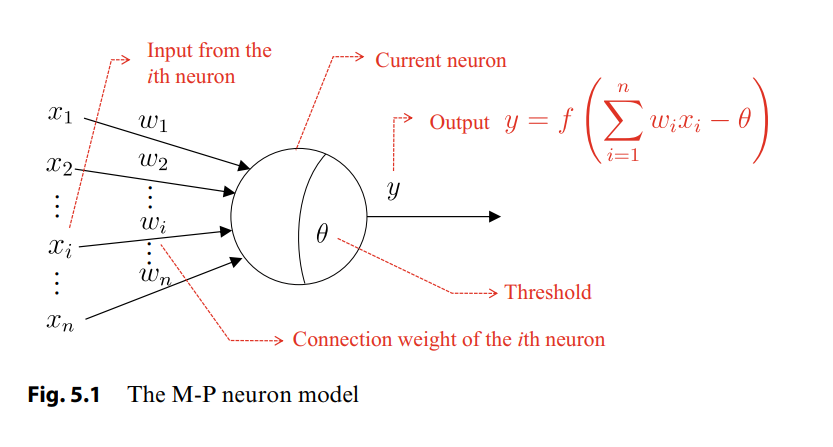
\includegraphics[width=6cm]{figure_neural_network.png}
	\caption{Beispiel eines einfachen künstlichen neuronalen Netzes. Quelle: \parencite{Zhou2021}}
\end{figure}

% Wie neuronale Netze lernen
Die Optimierung des Netzwerks geschieht durch eine Rückwärtsausbreitung (engl. \textit{backpropagation}), welche den berechneten Fehler rückwärts durch das Netz propagiert, um die Gewichte und Schwellenwerte um einen geringen Wert in die Richtung anzupassen, die den Fehler minimieren würde. ...

% Mathematik beschreiben; kann mehr oder weniger im Schnelldurchlauf
	% Softmax
	% Loss
		% Cross-Entropy
	% (Stochastic Gradient Descend)
	% (Backpropagation)
	% (Regularisierung)

\subsection{Convolutional Neural Networks} % Brauche ich das überhaupt? Als Beispiel?

% Kurze Definition
Ein Convolutional Neural Network (CNN) ist ein spezielles künstliches neuronales Netz, das hauptsächlich für die Bildklassifikation entwickelt wurde. Es verwendet Faltungsebenen, um ein Eingangsbild Schritt für Schritt in immer abstraktere “Feature Maps” zu verarbeiten.

% Architektur eines CNN
Die Architektur eines CNN besteht typischerweise aus mehreren Schichten, die in der folgenden Reihenfolge angeordnet sind:

\begin{enumerate}[]
	\item Eingabeschicht (Input Layer): Diese Schicht nimmt die Rohdaten auf, z.B. ein Bild in Form eines 2D-Arrays von Pixelwerten.
	\item Faltungsschicht (Convolutional Layer): Diese Schicht führt die eigentliche Faltung (Convolution) durch, indem sie einen Filter (Kernel) über das Eingabebild verschiebt und Punktoperationen durchführt. Das Ergebnis ist eine Feature-Map, die lokale Merkmale des Bildes extrahiert. Jeder Filter kann unterschiedliche Merkmale wie Kanten, Ecken oder Texturen erkennen.
	\item Aktivierungsschicht (Activation Layer): Nach jeder Faltungsschicht wird normalerweise eine Aktivierungsfunktion angewendet, um nichtlineare Eigenschaften des Netzwerks zu modellieren. Die häufig verwendete Aktivierungsfunktion ist die ReLU (Rectified Linear Unit), die alle negativen Werte auf Null setzt und positive Werte unverändert lässt.
	\item Pooling-Schicht (Pooling Layer): Diese Schicht reduziert die räumliche Dimension der Feature-Maps, was die Berechnungen effizienter macht und die Gefahr von Überanpassung (Overfitting) verringert. Die gängigsten Pooling-Methoden sind Max-Pooling (wählt den maximalen Wert in einem bestimmten Bereich) und Average-Pooling (berechnet den Durchschnittswert in einem bestimmten Bereich).
	\item Vollständig verbundene Schicht (Fully Connected Layer): Dies ist eine herkömmliche neuronale Netzwerkschicht, bei der jeder Neuron mit jedem Neuron der vorherigen Schicht verbunden ist. Sie kombiniert die extrahierten Merkmale, um das endgültige Ergebnis zu liefern, z.B. die Klassifikation des Bildes.
	\item Ausgabeschicht (Output Layer): In der letzten Schicht wird eine Aktivierungsfunktion wie Softmax verwendet, um die Wahrscheinlichkeitsverteilung der möglichen Klassen zu berechnen.
\end{enumerate}

\subsection{Out-of-Distribution Daten}

% Definition und Problematik
Wenn ein KI-Modell mit Daten konfrontiert wird, die außerhalb des Bereichs liegen, den es während des Trainings gesehen hat, spricht man von Out-of-Distribution (OOD) Daten. Es handelt sich also um Datenpunkte oder Muster, die sich signifikant von den Trainingsdaten unterscheiden. Dies kann zu Problemen führen, da das Modell möglicherweise nicht in der Lage ist, angemessene Vorhersagen oder Entscheidungen für diese ungewohnten Daten zu treffen. Stattdessen werden falsche Vorhersagen mit übermäßigem Vertrauen getroffen.

% OOD-Detection
Die Erkennung von OOD-Daten ist ein wichtiges Forschungsgebiet im maschinellen Lernen, da sie dazu beitragen kann, die Zuverlässigkeit und Sicherheit von KI-Systemen zu verbessern. Idealerweise sollte ein neuronales Netz höhere Softmax-Wahrscheinlichkeiten für In-Distribution-Daten und niedrigere Wahrscheinlichkeiten für OOD-Daten ausgeben. Durch Festlegen eines Schwellenwerts für diese Wahrscheinlichkeiten können Instanzen unterhalb des Schwellenwerts frühzeitig als OOD-Instanzen erkannt und entsprechend behandelt werden. In der Praxis kommt dieser Ansatz jedoch oft an seine Grenzen, da die Softmax-Wahrscheinlichkeiten nicht immer zuverlässig sind und das Modell auch für OOD-Daten hohe Wahrscheinlichkeiten ausgeben kann. Daher werden alternative Ansätze verwendet, wie etwa das Training eines binären Klassifikationsmodells zur Unterscheidung von In-Distribution und OOD-Daten.

\subsection{Datenaugmentation und Generalisierung}

% Definition und Zweck
Datenaugmentation ist ein wichtiger Schritt im Training von neuronalen Netzen, insbesondere bei begrenzten Datensätzen. Sie bezieht sich auf die künstliche Erweiterung des Trainingsdatensatzes durch Anwenden von Transformationen auf die vorhandenen Daten. Diese Transformationen können z.B. Rotation, Skalierung, Verschiebung, Spiegelung, Helligkeitsanpassung oder Rauschen sein. Das Ziel der Datenaugmentation ist es, das Modell robuster gegenüber Variationen in den Eingabedaten zu machen und die Generalisierungsfähigkeit zu verbessern.

% Beispiele
%\begin{figure}[]
%	\centering
%	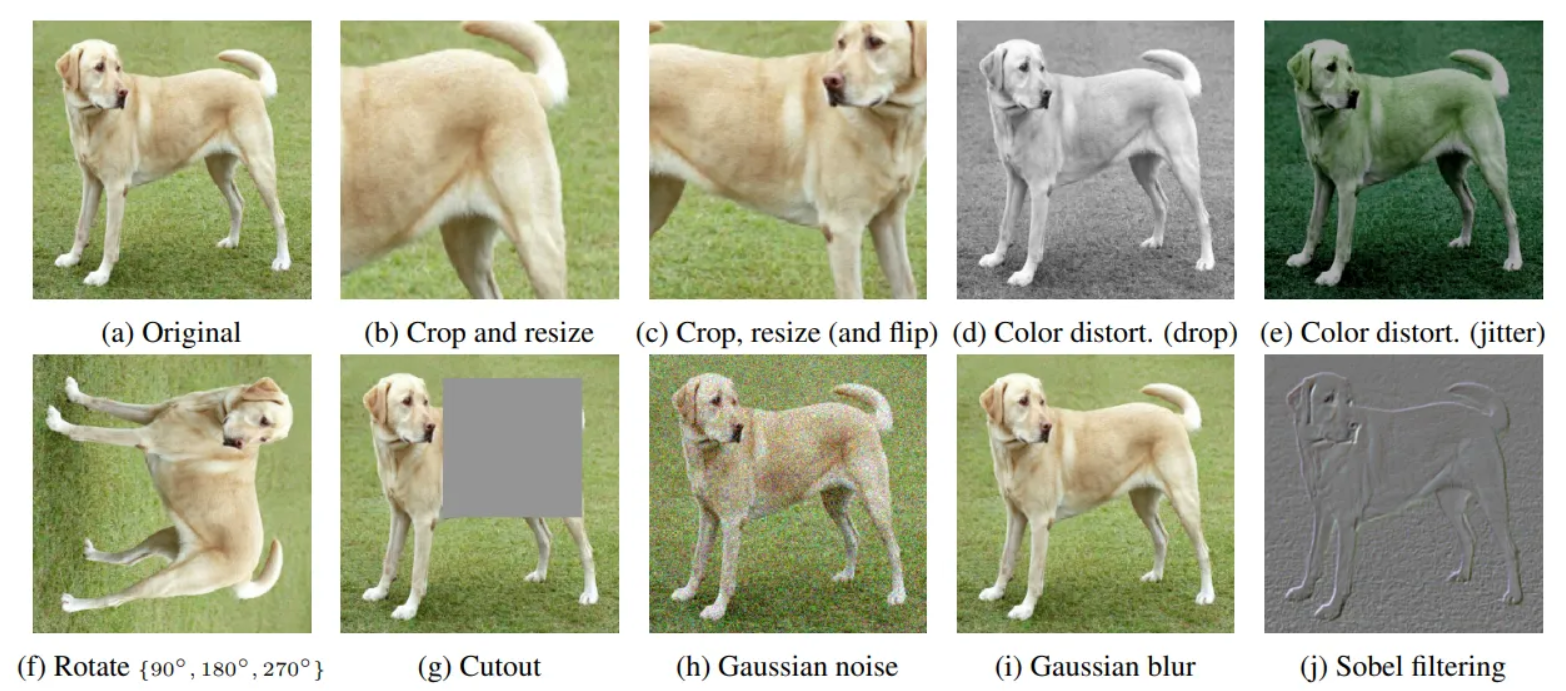
\includegraphics[width=6cm]{figure_data_augmentation.webp}
%	\caption{Beispiele für Datenaugmentationstechniken. Quelle: Thijs Kooi}
%\end{figure}

\section{Synthetische Daten}

% Anschließend an Datenaugmentation; Problematik der Datensammlung
% Abgrenzung synthetischer Datengenerierung zu Datenaugmentation
% (Vorteile und Herausforderungen synthetischer Daten)
% Fortschritte generativer Modellierung, Einleitung folgender Abschnitte

Während die Verfügbarkeit großer Datensätze für das Training von neuronalen Netzen ein entscheidender Faktor für den Erfolg von Deep Learning-Modellen ist, ist es oft schwierig, solche Datensätze zu sammeln, insbesondere in Domänen wie der Medizin oder der Robotik, wo die Daten rar und teuer sind \cite{}. In solchen Fällen können synthetische Daten eine nützliche Alternative oder Ergänzung zu echten Daten sein.

Synthetische Daten sind künstlich erzeugte Daten, welche die zugrundeliegenden Muster der realen Daten nachahmen. Sie können durch Simulation, Generierung oder Transformation von echten Daten erstellt werden.

...

\subsection{Variational Autoencoder}

...

\subsection{Generative Adversarial Networks}

...

\subsection{Stable Diffusion}

Unter Diffusion versteht man den Prozess der langsamen Vermischung von Partikeln oder Informationen über die Zeit. In der Physik beschreibt die Diffusionsgleichung die zeitliche Entwicklung der Dichte von Teilchen, die sich zufällig bewegen. Dieses Konzept fand erstmals im maschinellen Lernen Anwendung, als Jascha Sohl-Dickstein et al. 2015 das Konzept der Diffusion-Modelle einführten \parencite{}.

Bei Diffusion-Modellen handelt es sich um eine Klasse von generativen Deep Learning-Modellen, die in den letzten Jahren erhebliche Fortschritte erzielt haben. Im Trainingsprozess wird schrittweise die Struktur der Eingabedaten durch Hinzufügen von Rauschen aufgelöst. Das Modell wird dann darauf trainiert, das ursprüngliche Bild aus dem verrauschten Bild zu rekonstruieren.

...

\subsection{DA-Fusion}

...

\section{Contrastive Learning}

% Ursprung Contrastive Learning
% Einführung in die Grundprinzipien
% Unterscheidung zwischen Self-Supervised *Instance* Discrimination, Supervised *Class* Discrimination (Keshtmand2022)

...

\subsection{Unsupervised Contrastive Learning}

% Annotation von Daten ist sehr aufwendig
% Contrastive Learning als Unsupervised Alternative
	% Kann auch als Self-Supervised betrachtet werden, da durch die Kontrastierung der Daten eine Art von Supervision entsteht
% Vor allem deshalb so vielversprechend, weil die erlernten Repräsentationen eine bessere Generalisierung und Robustheit gegenüber Adversarial Attacks aufweisen (Liu2021)
% SimCLR (Chen2020) als prominentes Beispiel
	% Einführung eines Projection Heads, welcher die Repräsentationen der Eingabedaten in einen höherdimensionalen Raum projiziert
	% Verwendung von Data Augmentation, um die Robustheit der Repräsentationen zu verbessern
	% Größere Batch Sizes und längere Trainingszeiten begünstigen die Lernfähigkeit des Modells
	% Zudem ist besonders die Wahl von hard negatives entscheidend für den Erfolg des Modells
% Eine neuere Variante: StableRep (Tian2023)
	% Verwendung von synthetischen Daten aus T2I-Modellen, insbesondere Stable Diffusion
	% Verwendet Bilder, die aus dem selben Prompt generiert wurden, als positive Beispiele voneinander
	% Kann mit den richtigen Einstellungen auch mit Training nur auf synthetischen Daten die Leistung von SimCLR übertreffen
	% Noch bessere Ergebnisse bei Einbeziehung von Textsupervision

...

\subsection{Supervised Contrastive Learning}

% Erweiterung der Contrastive Learning-Methode durch Verwendung von Label-Informationen
% SupCon (Khosla2020)
	% Weiterentwicklung der Loss-Funktion, die mehrere positiv-Beispiele pro Anchor-Sample berücksichtigt und das Contrastive Learning auf das Supervised Setting anpasst
	% Eine rein naive Anpassung wird aber um einige wünschenswerte Anpassungen erweitert
		% Es wird nicht ein Anchor, ein positiv-Beispiel und viele negativ-Beispiele verwendet; stattdessen kommen im Supervised Contrastive Learning auch viele positiv-Beispiele pro Batch zum Einsatz
		% Die *vielen* positiv-Beispiele werden zudem nicht mehr als Augmentationen des Anchor-Samples generiert, sondern als Samples der gleichen Klasse herangezogen
		% So soll auch die Notwendigkeit des Hard-Negative Minings reduziert werden
		% Trotzdem wird gezeigt, dass der resultierende Loss sowohl von hard-negatives wie auch hard-positives profitiert
		% Verwendung des Mittelwertes der positiven Repräsentationen stabilisiert das Training und führt zu einer verbesserten Leistung
% Generalized SCL (Kim2022)
	% Label als Distribution
% Supervised Contrastive Learning with Hard Negatives (Jiang2022)
	% Zusätzliche Einschränkung des Negative Samplings für Auswahl von Hard Negatives (Nähe im Repräsentationsraums)

...

\section{Integration von DA-Fusion und Supervised Contrastive Learning}

% Rückverweis auf Anwendungsfall
% Einleitung für den vorzustellenden Ansatz
...

\subsection{Herausforderungen bei der Generierung synthetischer Daten}

% Herausforderungen bei der Generierung synthetischer Daten
	% Komplexe Objekte
	% Feine Unterschiede zwischen Klassen
	% Wenig Variation
	% (Detaillierte Meta-Informationen, Multimodalität)
	% Risiko der Fehlklassifikation von OOD-Daten
% Welche Anforderungen ergeben sich?
	% Hohe Kontrolle über die Generierung der synthetischen Daten; Genauigkeit
	% Trotzdem Verbesserung der Generalisierungsfähigkeit
	% Verbesserung der OOD-Detektion
...

\subsection{Potenzial von DA-Fusion zur kontrollierten Augmentation}

...

\subsection{Supervised Contrastive Learning zur Verbesserung der Generalisierung und Robustheit}

...

\subsection{“Schlechte” synthetische Daten als negativ-Beispiele?}

% Forschungslücke bei der Integration von synthetischen Daten im Contrastive Learning
	% StableRep
		% Stable Diffusion "off-the-shelf" ist nicht akkurat genug
			% Objekte zu komplex
			% Zu ähnlich; feine Unterschiede
		% Auch die gleichbleibenden Hintergründe sind fatal
		% Außerdem: Unsupervised
	% Supervised Contrastive Learning mit Hard Negatives
		% Gute Strategie für Negative-Sampling
		% Aber keine synthetischen Daten
% Was wenn: Anstatt Negatives aus Nähe im Darstellungsraum zu samplen, Near OOD-Augmentationen aus Anchor-Klasse?
% DA-Fusion zur Generierung von ID- und Near OOD-Daten
	% Einfach den strength-Parameter der DA-Fusion-Augmentationen erhöhen
	% Bei der Generierung die Maske verwenden, damit die Hintergründe gleich bleiben
% Supervised Contrastive Learning mit eigener Sampling-Strategie für Near OOD-Negatives
...

\subsection{Potenzielle Vorteile und Herausforderungen}

% Bessere Generalisierung
	% SimCLR profitierte besonders von hard negatives, um gute Repräsentationen zu lernen
	% OOD-Augmentationen müssen an sich keine spezifischen Klassen akkurat repräsentieren, sind aber dennoch nah genug an den echten Daten, um dessen Repräsentationen zu verbessern
% Bessere OOD-Detektion
	% OOD-Detection profitiert von einer guten Repräsentation der Daten, um die Distanz zwischen In-Distribution und OOD-Daten zu maximieren
	% Near OOD-Negatives sind nah genug an den echten Daten, um die Repräsentationen zu verbessern, aber dennoch OOD genug, um die Distanz zu maximieren
...